\chapter{Improving the Radial Velocity Precision of Keck/HIRES}\label{chap:keck}


%%%%%%%%%%%%%%%%%%%%%%%%%%%%%%%%%%%%%%%%%%%%%%%%%%%%%%%%%%%%%%%%%%%%%%%%%%%%%%%%
\section{Introduction and Background}

This is about Keck/HIRES.


%%%%%%%%%%%%%%%%%%%%%%%%%%%%%%%%%%%%%%%%%%%%%%%%%%%%%%%%%%%%%%%%%%%%%%%%%%%%%%%%
\section{Effects of Telluric Contamination and Remedies}\label{keck:sec:telluric}

% main text for the telluric section in keck.tex
%%%%%%%%%%%%%%%%%%%%%%%%%%%%%%%%%%%%%%%%%%%%%%%%%%%%%%%%%%%%%%%%%%%%%%%%%%%%
%%%%%%%%%%%%%%%%%%%%%%%%%%%%%%%%%%%%%%%%%%%%%%%%%%%%%%%%%%%%%%%%%%%%%%%%%%%%
\subsection{Introduction}\label{keck:telluric:intro}

The first exoplanets around main-sequence stars were discovered by the
radial velocity (RV) method, where precise Doppler spectroscopy
measures the wavelength shift of the host stars induced by the
gravitational pull of the planets \citep{1988ApJ...331..902C,
  1989Natur.339...38L, 1993ApJ...413..339H, 1995Natur.378..355M,
  1996ApJ...464L.153B}. Since then, the RV method has discovered
hundreds of planetary systems (see exoplanets.org; \citealt{eod2014})
and contributed to numerous confirmation and characterization of
exoplanets discovered by the transit method (e.g., for
\kepler\ follow-up observations; \citealt{Marcy2014}).

The current best RV precision is around 1~m/s \citep{eprv2015},
attainable via two wavelength calibration methods in the optical band:
ThAr lamp emission line calibration (e.g., ELODIE and HARPS;
\citealt{elodie, harps-s}; $\sim$400-690~nm) and iodine cell
absorption line calibration (e.g., Keck/HIRES and Magellan/PFS;
\citealt{butler1996, 2010SPIE.7735E..53C}; $\sim$500-620~nm). The
major obstacles for achieving a higher RV precision are: stellar
activity induced RV signals, instrumental effects, telluric
contamination, and limitation in data analysis \citep{eprv2015}.

Traditionally, telluric contamination is not considered as problematic
for precise RV in the optical. It is certainly a sever source of
spectral contamination and a bottleneck for achieving higher RV
precision in the near infra-red (NIR) region (e.g.,
\citealt{2010ApJ...713..410B}), where a large number of deep water and
methane lines reside. However, there is only a small wavelength
range in the optical that has deep telluric lines, and typically such
regions are simply thrown out for the purpose of precise RV analysis,
either by giving them zero weights in the cross correlation masks (for
ThAr calibrated spectra, e.g., \citealt{2002A&A...388..632P}) or
flagging them as bad pixels (for iodine calibrated spectra, e.g., for
Keck/HIRES).

Recently, the works by \cite{artigau2014} and \cite{cunha2014} have
characterized and mitigated the effects of telluric contamination in
the precise RV data taken by the ThAr-calibrated HARPS-S.
\cite{cunha2014} focuses on the issues with ``micro-telluric" lines
(shallow telluric absorption lines with $<1$-3\% depths), which are
recognized for the first time. \cite{cunha2014} fit and then divide
out the telluric lines in the observed spectra using synthetic
telluric spectra generated by the LBLRTM package (Line-By-Line
Radiative Transfer Model, \citealt{lblrtm}; with line lists from
HIgh-resolution TRANsmission molecular absorption database, or HITRAN,
\citealt{hitran2013}) and also TAPAS \citep{tapas}, which is a more
user-friendly but less flexible package wrapper using LBLRTM. They
concluded that the micro-tellurics have an impact (defined as RMS of
difference between RVs before and after micro-telluric removal) of
$\sim$10-20 cm/s for G stars observed with low to moderate air masses,
but the impact can be substantial in some cases to up to $\sim$0.5-1
m/s.

\cite{artigau2014} uses principal component analysis (PCA) to
empirically correct for telluric lines in HARPS-S data (both
micro-tellurics and the deep lines in the $\sim$630~nm region), and
combined PCA with rejection masking, they reduced the RV RMS by
$\sim$20~cm/s (and more significantly for the $\sim$630~nm
region). More recently, \cite{2016AAS...22713719S} characterized the
effects of telluric contamination and effectiveness of some typical
remedies (masking and modeling) for emission line-calibarated spectra
for the optical, broad optical (300-900~nm), and NIR. Their conclusion
for the optical region is similar to the results in \cite{artigau2014}
and \cite{cunha2014}.

This paper characterizes and corrects for the adverse effects of
telluric contamination under the context of iodine-calibrated precise
RV, especially for the micro-telluric lines. ZZZ We first describe our
methodology for characterizing the effects of tellurics in
Section~\ref{keck:telluric:method}, then... ZZZ


%----------------------------------------------------------------
% Plot showing micro-telluric lines
% made by ~/Exo../Keck../plots_general/spec_plot.pro
\begin{figure}
\includegraphics[scale=0.5]{telluric/tellurics_all.eps} 
\caption{Telluric lines in the iodine region are mostly shallow water
lines, with some moderately deep water lines near 5900\AA\ and very
deep oxygen lines near 6300\AA. The insert plot is showing the
pervasiveness of micro-telluric lines, i.e.~$\leq$1--3\% in depths.
\label{telluric:fig:telluric}}
\end{figure}
%----------------------------------------------------------------



%%%%%%%%%%%%%%%%%%%%%%%%%%%%%%%%%%%%%%%%%%%%%%%%%%%%%%%%%%%%%%%%%%%%%%%%%%%%
%%%%%%%%%%%%%%%%%%%%%%%%%%%%%%%%%%%%%%%%%%%%%%%%%%%%%%%%%%%%%%%%%%%%%%%%%%%%
\subsection{Impacts of Micro-tellurics on RV Precision}\label{keck:telluric:method}

% why Keck, why 185144 and 10700
To evaluate the impacts of micro-tellurics (referred to often simply
as ``tellurics'' below), we performed end-to-end simulation of \keck\
data and analysis process on RV standard stars in order to isolate
error sources. We use \keck\ data to for our study because Keck has
the highest RV precision among all iodine-calibrated spectrometers,
and it also has long observing baselines on a number of RV standard
stars. RV standard stars are bright and quite stars which do not host
known planets, and thus exhibit the smallest RV variation in both
short term and long term. Their data are often good diagnostic tools
for identifying RV systematics. For our study, we used and simulated
\keck\ RV spectra on two standard stars, $\sigma$ Draconis (HD 185144)
and $\tau$ Ceti (HD 10700), which are benchmark classics in precise RV
work.

% more on the two stars 
HD 185144 (spectral type G9V, per Simbad) has 712 \keck\ observations,
with RV RMS $=$ 2.57 m/s, and it has a relatively small barycentric
velocity (often referred to as the barycentric velocity correction, or
BC; see Chapter~\ref{chap:doppler}) span, $[-4.7,\ 4.6]$ km/s, because
it is near the north ecliptic pole. HD 10700 (spectral type G8.5V) has
623 observations, with RMS $=$ 3.05 m/s, and its BC span is $[-27.8,\
26.8]$ km/s. The RV RMS numbers quoted here come from reductions using
our version of CPS Doppler pipeline, and they are larger than the RMS
values from the most up-to-date CPS pipeline due to some recent
improvements in the CPS version. The most recent CPS inventory (as of
April 2016) also has a few new observations on these two stars.


%%%%%%%%%%%%%%%%%%%%%%%%%%%%%%%%%%%%%
\subsubsection{Methodology}\label{keck:telluric:method}

We simulated Keck observations on sig Dra and tau Ceti by using
synthetic stellar spectra of their respective spectral types (?) using
SME (ZZZ cite Valenti and Fischer). We simulated one spectrum for each
actual observed spectrum taken at Keck through the CPS programs. The
synthetic stellar spectra is multiplied with the iodine atlas to
create the standard iodine$+$ star RV observations. The multiplied
spectrum is then multiplied with the blaze function and convolved with
the observed spectral PSF, both derived from real observations for
each night. Poisson noise is added.

We then forward model the simulated spectra to extract RVs using the
CPS Keck code (ZZZ cite Johnson and Howard). We used the synthetic
stellar spectrum as the input stellar template. In reality, stellar
templates are derived from observed stellar spectra via deconvolution,
which would introduce additional errors. Using the same synthetic
stellar spectrum would eliminate such errors and isolate the problem
to telluric lines only.

We ran two sets of simulations: control and contaminated. In the
control, we only had stellar spectrum and iodine spectrum. In the
contaminated, we added in simulated telluric lines in the simulated
observed spectrum. The telluric lines were generated using TERRASPEC
(ZZZ cite Bender). We adopted the typical Mauna Kea atmospheric
condition (temperature and pressure profiles) and typical oxygen
column density (which in realiaty flucturate very little anyway). For
simplicity, we assumed the same water column density for every
observation, which is pwv$=1$mm, a little bit humid than a typical
Mauna Kea night (true? I think this is actually pretty typical). The
pair of simulated control and contaminated spectra have the same added
Poisson noise, and therefore any RV differences derived from these two
sets of simulation would reveal the net effect of telluric
contamination.


%%%%%%%%%%%%%%%%%%%%%%%%%%%%%%%%%%%%%
\subsubsection{Results}

%----------------------------------------------------------------
% Telluric effect, no photon noise
% plot made by ~/Exo.../Keck.../simulate.../msplot.pro
\begin{figure}
\subfloat{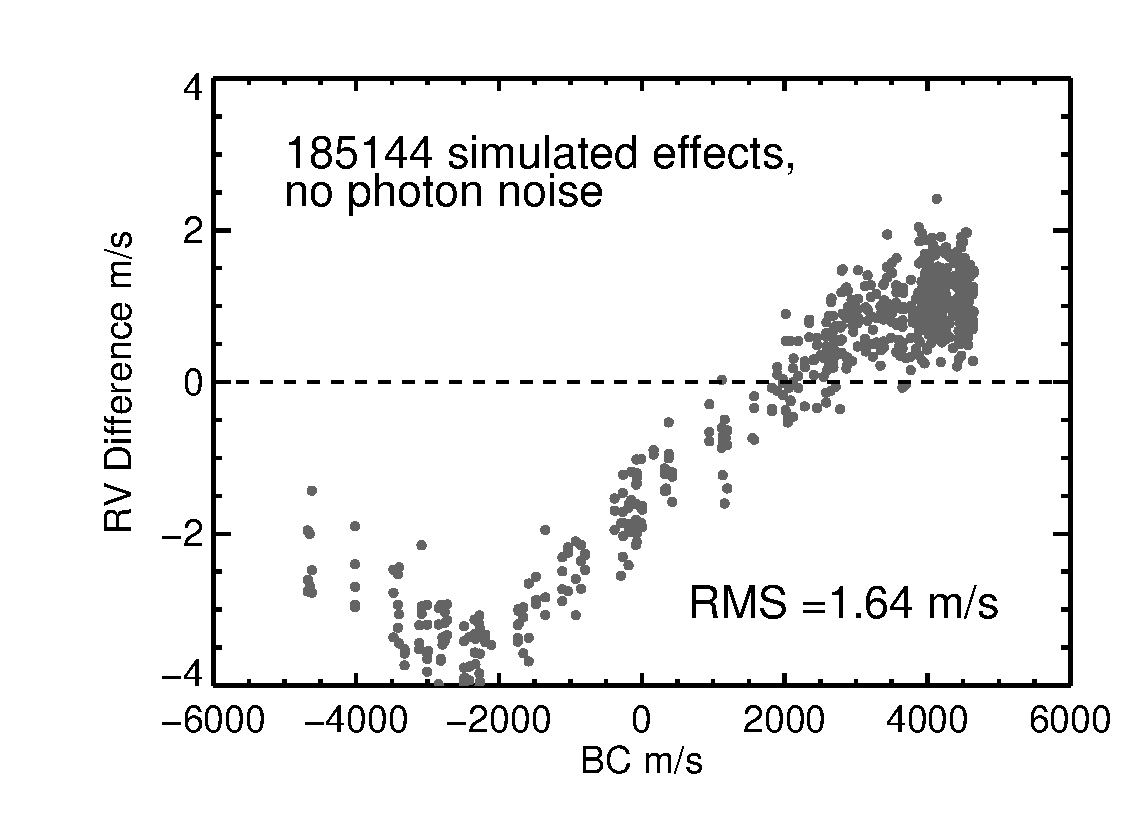
\includegraphics[scale=0.38]{telluric/185144-rv-bc-rja01-rjb01.eps}}\
\subfloat{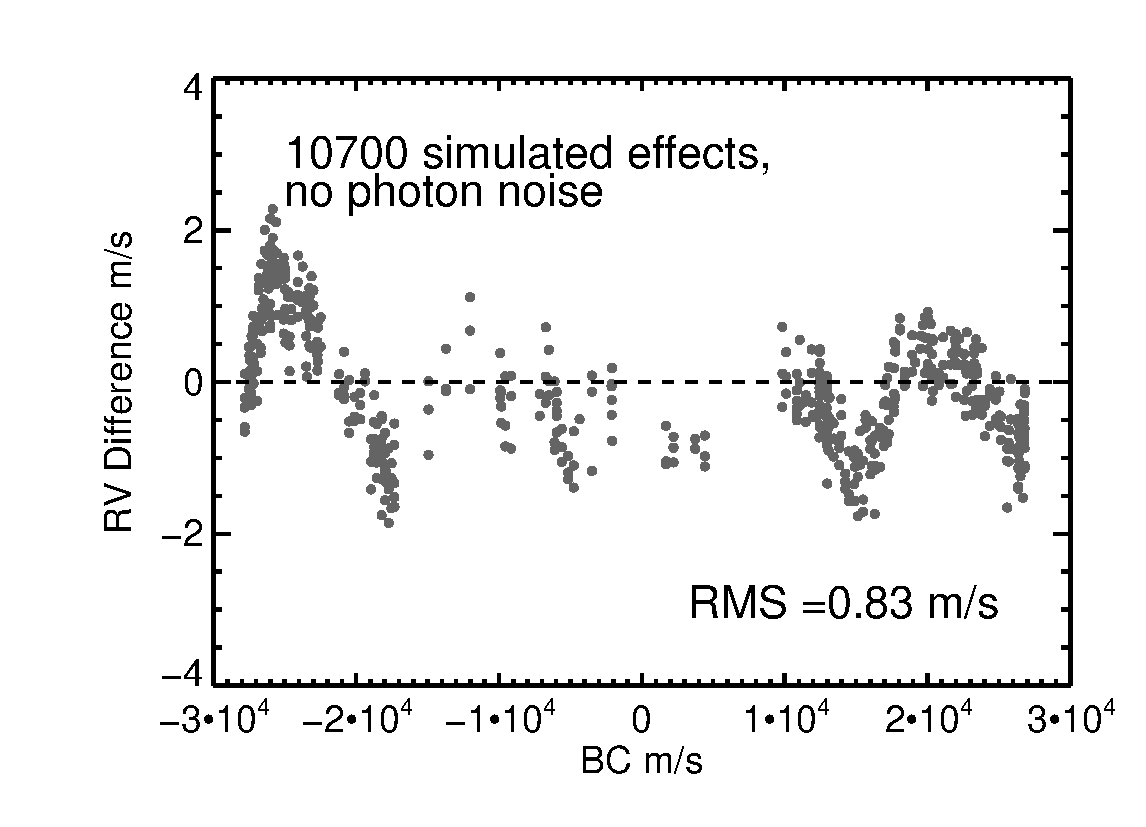
\includegraphics[scale=0.38]{telluric/10700-rv-bc-rja01-rjb01.eps}}\
\subfloat{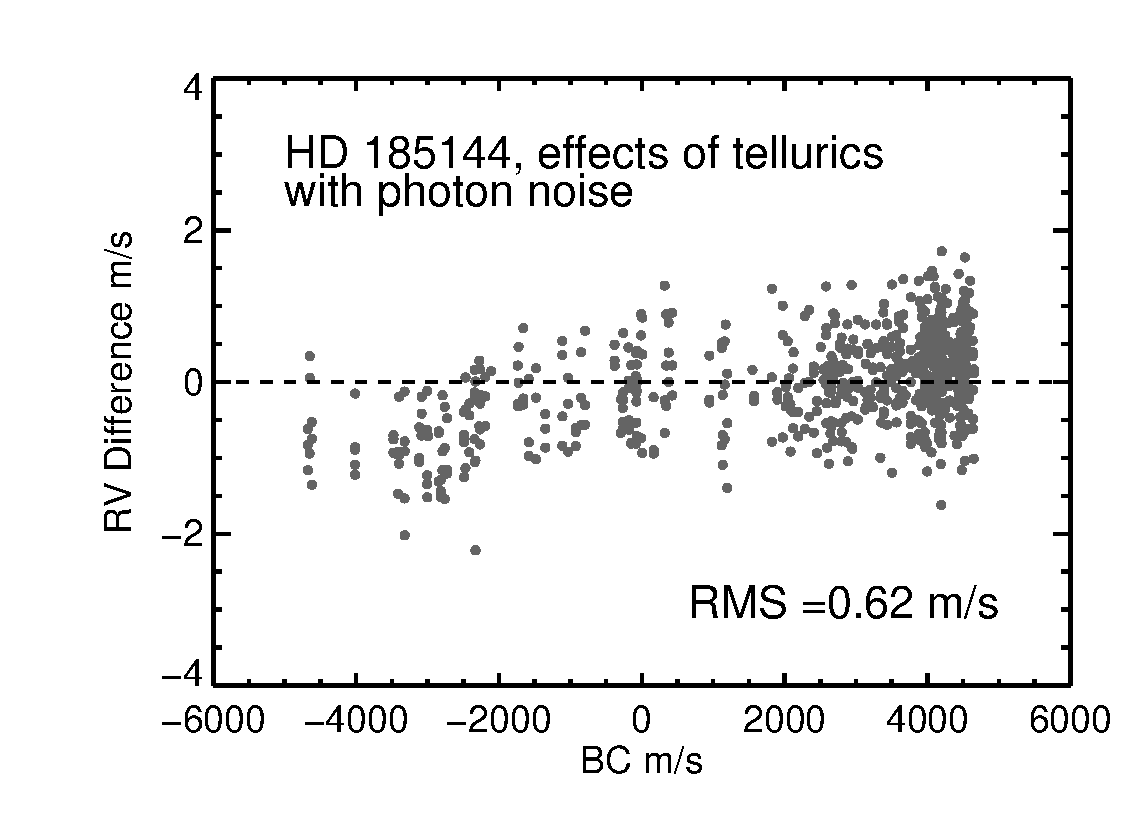
\includegraphics[scale=0.38]{telluric/185144-rv-bc-rjc01-rjd01.eps}}\
\subfloat{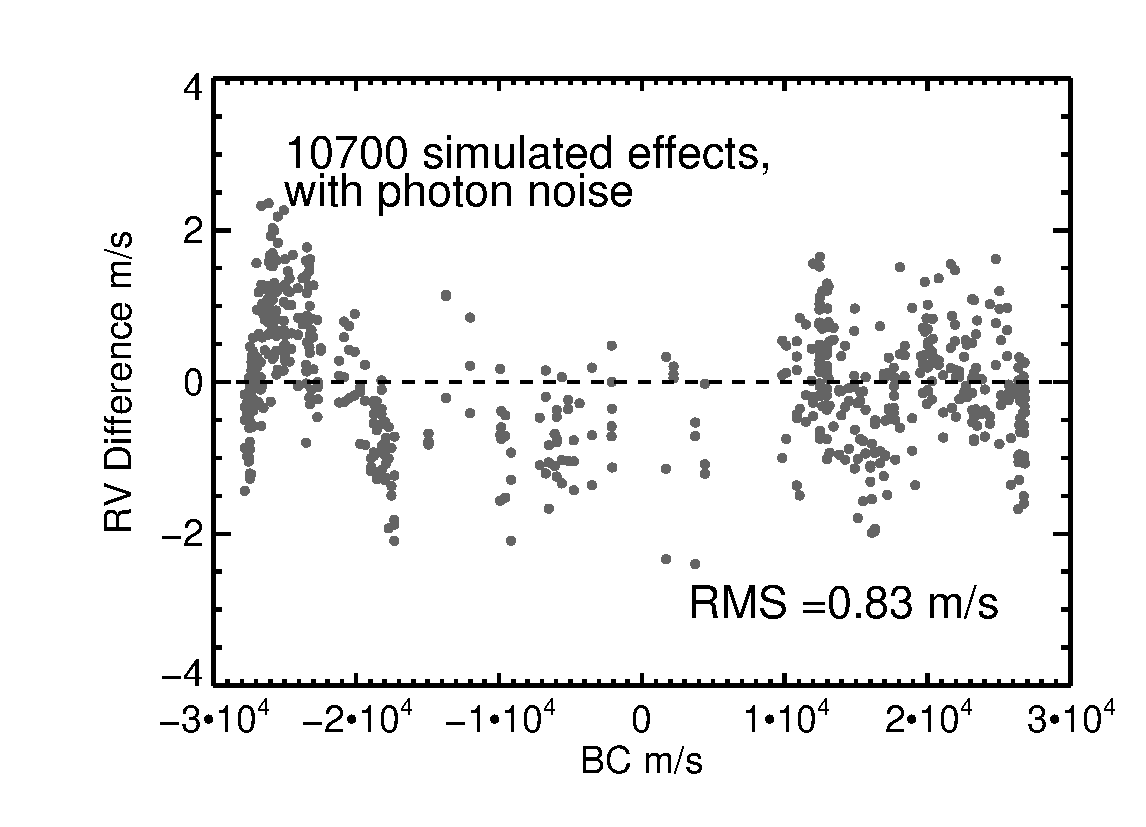
\includegraphics[scale=0.38]{telluric/10700-rv-bc-rjc01-rjd01.eps}}\
\subfloat{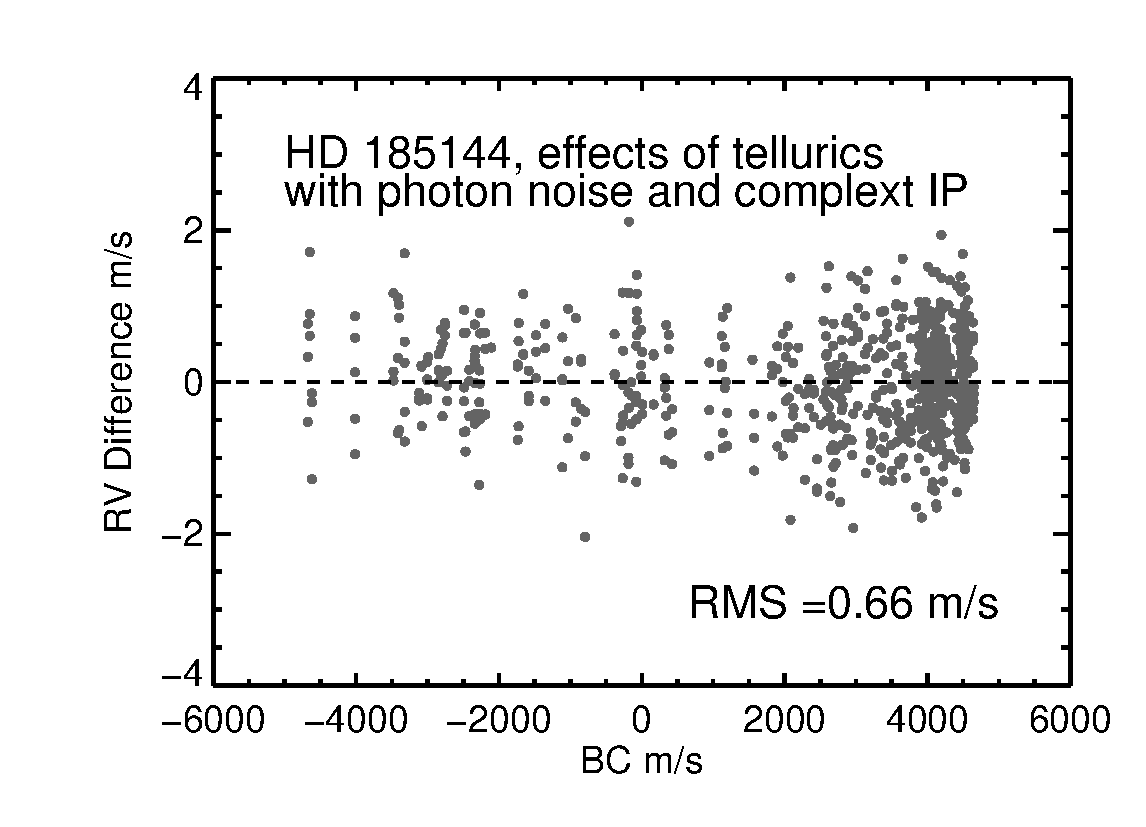
\includegraphics[scale=0.38]{telluric/185144-rv-bc-test0-test1.eps}}\
\subfloat{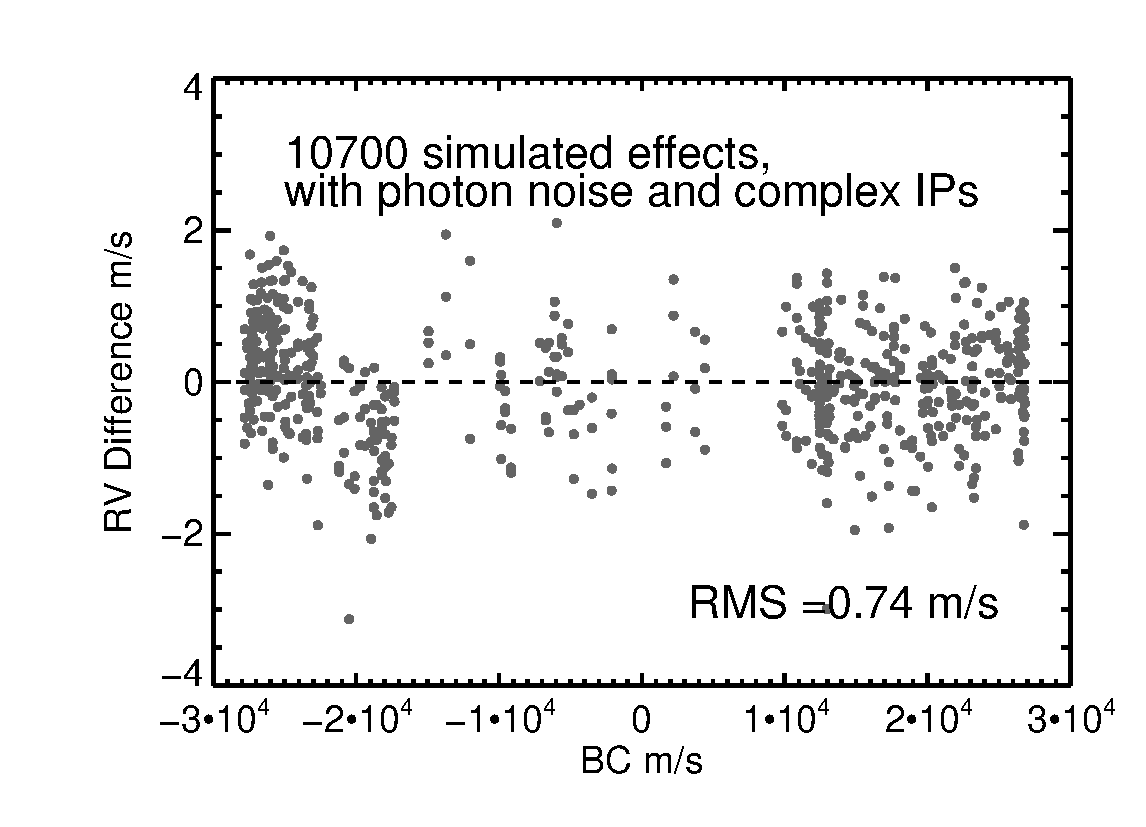
\includegraphics[scale=0.38]{telluric/10700-rv-bc-test0-test1.eps}}\
\caption{Effects of telluric lines manifested as correlation between
  RV and BC. Each point represents the difference in RV estimates for
  a pair of simulated spectra: one without telluric absorption, and
  one with telluric absorption on top of the stellar and iodine
  spectra. {\bf Top 2 panels:} To isolate the effects of telluric
  lines, the simulated spectra used for this plot do not have Poisson
  noise added, and they have simple one-component Gaussian IPs which
  have fixed width and thus the IP parameters are all fixed to the
  true values in the RV extraction. {\bf Middle 2 panels:} same as the
  top panels, but for simulated spectra with Poisson noise (same noise
  for the telluric and non-telluric spectrum pairs; and still the same
  simple IPs). {\bf Bottom 2 panels:} same as above, but for simulated
  spectra with Poisson noise and complex IPs that are similar to the
  ones in actual observations. IP parameters are not fixed in this
  case, so the code is fitting 12 additional parameters for the IP on
  top of the 3 for wavelength solution and Doppler shift (see
  Chapter~\ref{chap:doppler} for more details on the code).
\label{telluric:fig:sim}}
\end{figure}
%----------------------------------------------------------------


Micro-tellurics in the iodine region introduces RMS$=0.6$ m/s scatter
for GK stars (RV systematic error added in quadrature). Leaving
untreated, this would define the precision floor.

Additionally, it manifests as spurious signal at periods of a sidereal
year and harmonics, with an amplitude of 20 cm/s. This would affect
our ability to detect super-Earth in the habitable zone of GK stars
(Earth's signal is 8 cm/s). We have seen such spurious signal in Keck
data on many stars, and telluric contamination is one of the
contributing factors (see discussion for other factors).

For M stars... (probably worse)


%%%%%%%%%%%%%%%%%%%%%%%%%%%%%%%%%%%%%%%%%%%%%%%%%%%%%%%%%%%%%%%%%%%%%%%%%%%%
%%%%%%%%%%%%%%%%%%%%%%%%%%%%%%%%%%%%%%%%%%%%%%%%%%%%%%%%%%%%%%%%%%%%%%%%%%%%
\subsection{Remedies and Effectiveness}

There are several ways to remedy the adverse effects of telluric lines
on RV precision and accuracy: masking, modeling, or a combination of
both. HARPS works...

\subsubsection{Masking is an ineffective solution}

%----------------------------------------------------------------
% Table: RV RMS for various simulations
\renewcommand{\arraystretch}{1.2} % more row spacing for the table
\begin{deluxetable}{ccl}
\tabletypesize{\scriptsize}
\tablecaption{RV RMS for Simulations with Poisson Noise and Complex IP 
\label{telluric:tab:rmsmasking}}
\tablewidth{320pt}
\tablehead{
  \colhead{HD 185144} & \colhead{HD 10700} & \colhead{Simulation Conditions}
}
\startdata
1.26 m/s & 1.34 m/s & No tellurics \\
1.35 m/s & 1.42 m/s & With tellurics \\
1.35 m/s & 1.39 m/s & No tellurics, but masking telluric pixels \\
1.37 m/s & 1.43 m/s & With tellurics, and masking telluric pixels
\enddata
\end{deluxetable}
%----------------------------------------------------------------

% what do I mean when I talk about masking?
The simplest solution is to mask out telluric lines in the spectrum,
which means, in practice, locate the telluric-contaminated pixels and
flag them as bad pixels in the observed spectrum so that the
least-$\chi^2$ fitter will ignore them. For \keck\ or any
iodine-calibrated RV reduction, this also means masking out the
regions corresponding to locations of telluric lines in the
deconvolved stellar reference spectrum -- because the stellar
reference spectrum was taken at a different BC, the telluric lines
therein are shifted with respect to the ones in the epoch observation
as we try to match up the stellar lines in observed and reference
spectra. This ``double masking'' procedure is illustrated in
Figure~\ref{telluric:fig:dsstmask}. This is done ``dynamically'' in
the fitting process, in the sense that, for each iteration in the
least-$\chi^2$ minimization process, the contaminated pixels are
located according to the current wavelength solution parameters in
this fitting iteration. The wavelength solution changes from iteration
to iteration, and thus the masked pixels can change too.

%----------------------------------------------------------------
% Double masking of telluric lines
% plot made by converting pdf to eps. pdf comes from slides of CfASSP
% seminar talk, which can be found in ~/Ex.../Professional../..CfASSP../.
\begin{figure}
\subfloat{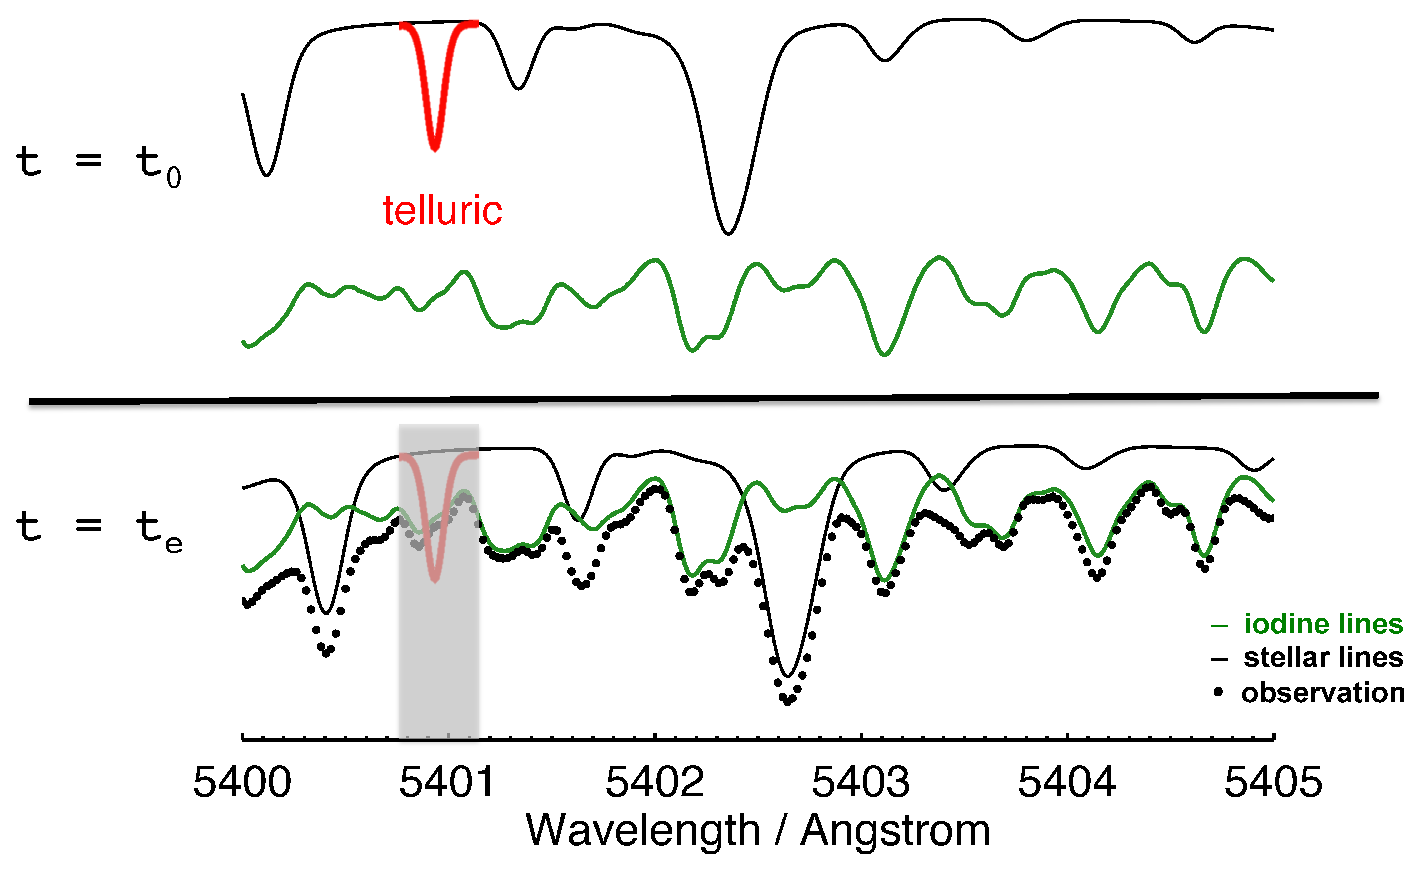
\includegraphics[scale=0.5]{telluric/dsst-mask1.eps}}\\
\subfloat{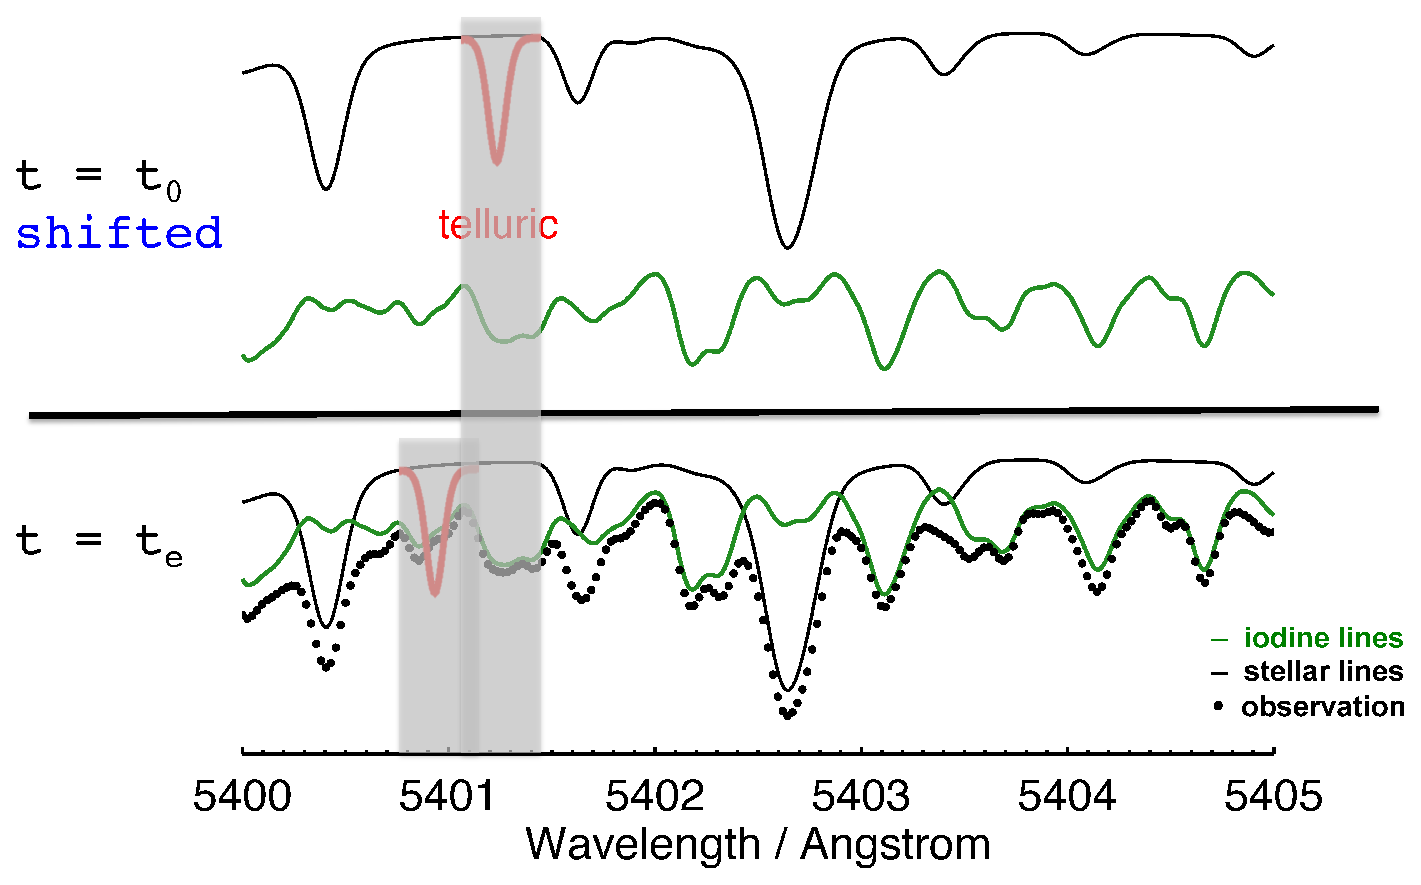
\includegraphics[scale=0.5]{telluric/dsst-mask2.eps}}
\caption{Illustration for how we mask telluric contaminated
pixels. The top panel shows how we mask the telluric lines (red solid
lines) in the epoch observation taken at $t=t_e$. The bottom panel
shows why we also need to mask pixels associated with telluric lines
in the deconvolved stellar reference spectrum taken at epoch $t=t_0$
and being shifted in order to model the observation.
\label{telluric:fig:dsstmask}}
\end{figure}
%----------------------------------------------------------------


% simulations and results
To investigate the effectiveness of masking, we performed RV
extraction on simulated spectra with or without telluric lines
injected and with or without masking (all with Poisson noise and
complex IP to mimic real observations as much as possible). For
stellar reference spectrum, we used the synthetic spectrum with
telluric lines. The results are tabulated in
Table~\ref{telluric:tab:rmsmasking}. In terms of improving RV
precision or reducing RV RMS, masking is very ineffective. The
additional errors it introduces diminish its merits. On the other
hand, masking does improve the accuracy to some degree: for example,
masking does remove the downward RV trend seen in HD 10700 data on the
bottom right plot of Figure~\ref{telluric:fig:sim} in the BC range
$[-3\times10^4,\ -2\times10^4]$ m/s. However, masking is an
ineffective way to mitigate the effects of telluric contamination
overall, especially since the RV errors and RV-BC trends are dominated
by photon noise and algorithmic errors (and other types of errors too
in real observations).

% why simple masking would not work for high precision/accuracy
So why masking does not work? First of all, it complicates the
$\chi^2$ surface and ``breaks'' the L-M fitter. Due to the ``dynamic''
nature of the mask mentioned above, the degrees of freedom for fitting
could change, because some telluric lines may shift in and out of this
spectral chunk as the wavelength solution changes. This would make the
fitter harder to converge or may create more loci for the fitter to
get stuck in, causing additional errors. Furthermore, masking is
throwing away iodine and stellar content embedded in these pixels
too. Finally, to ``mask'' the telluric lines out, one needs to pick a
flux threshold for the masks. This threshold must maintain a balance
between masking too much (throwing away too much iodine and stellar
information) and too little (leaving shallow telluric lines and line
wings untreated). In our study, we have chosen a flux threshold of
0.3\%, which means any pixel with telluric absorption deeper than
0.3\% will be masked (reference telluric spectrum is generated by
TERRASPEC at an altitude of 70$^{\degree}$, meaning deep oxygen lines,
and with precipitable water vapor (pwv) 0.8~mm, a little more than
typical \keck\ humidity). This masks 11\% of the spectral domain,
which is quite substantial and is very damaging to the RV precision,
but is almost the minimal amount of masking required to achieve some
RV accuracy improvement.

% how about masking in real observations?
We also applied telluric masking in RV reduction for real
observations, and saw no improvement over RV precision or
accuracy. This is because other effects dominate over telluric
absorption, as mentioned above, such as photon and algorithmic errors
and especially deconvolution errors in stellar reference spectrum,
which we will touch on in Section~\ref{keck:telluric:future} and
discuss in more detail in Section~\ref{keck:sec:dsst}.

% summarize
To summarize, masking sounds like a simple solution to the problem of
micro-telluric contamination, but it is actually complicated to
implement (for iodine-calibrated RV reduction) and it is ineffective
in terms of improving RV precision. We do not recommend masking as a
remedy for treating micro-telluric lines in iodine-calibrated RV
work. We believe the most effective way is to forward model telluric
lines, and combine that with some ``masking'' for deep or troublesome
telluric lines, which we discuss in the next subsection.

\subsubsection{How precisely does one need to model the tellurics?}


%----------------------------------------------------------------
% NEID Plot showing how much you need to model tellurics
\begin{figure}
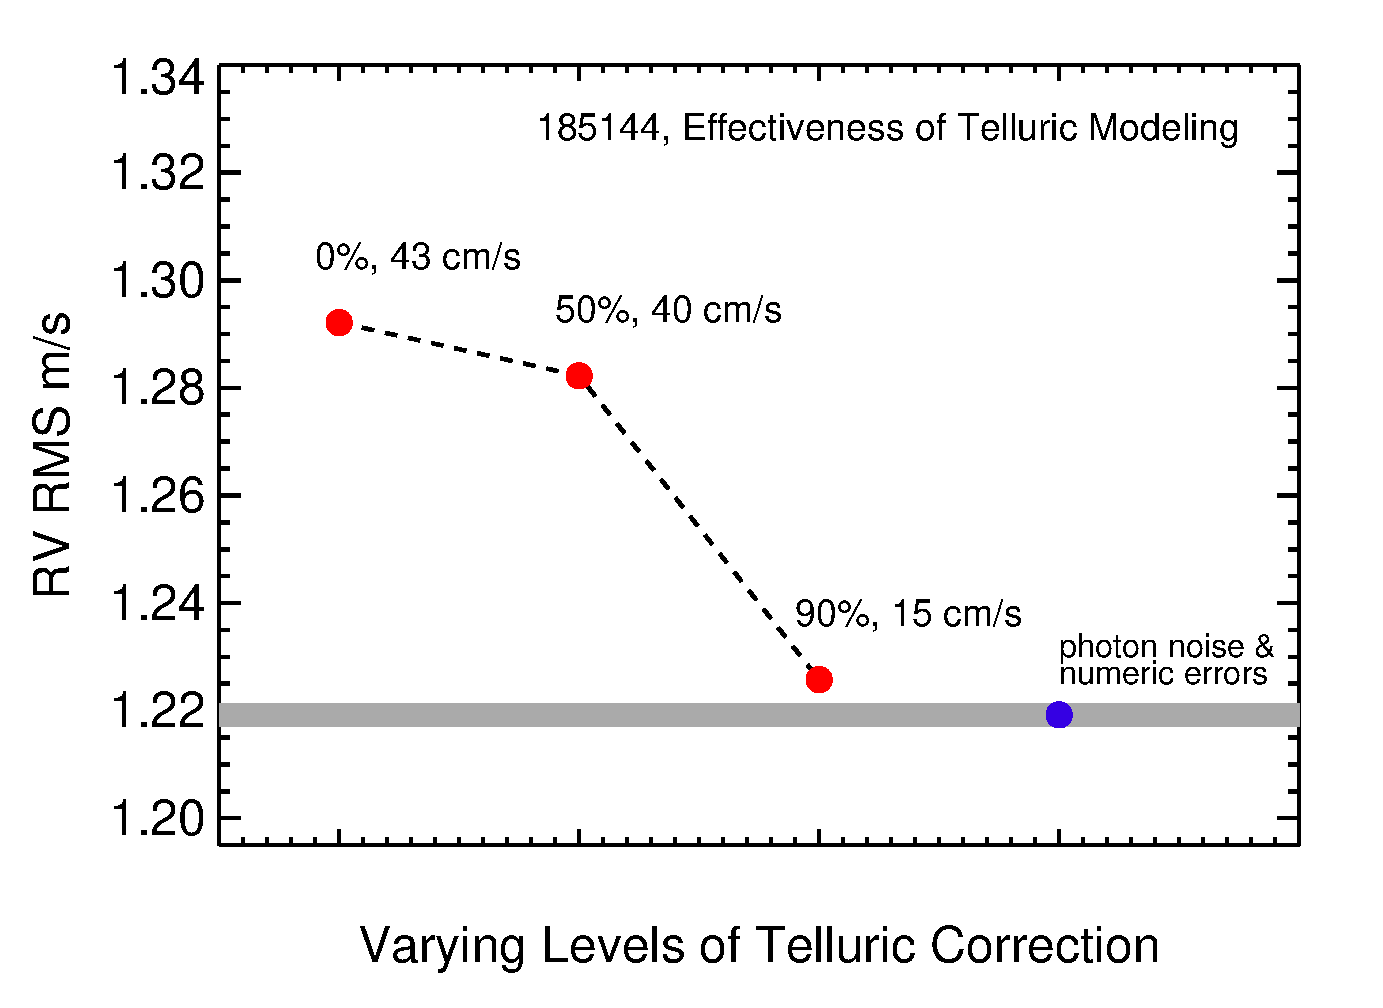
\includegraphics[scale=0.5]{telluric/neid.eps} 
\caption{Improvements in RV RMS for different ``level" of telluric
  modeling/removal. For example, the mid point labeled with ``50\%, 33 cm/s"
  means that if you model your telluric absorption lines to 50\% of
  their original depths, the effects of the residual telluric
  absorption will add 33 cm/s in quadrature to your final RV RMS. The
  blue point marks the RV RMS for simulations with Poisson noise and
  complex IP on HD 185144, which represents the photon-limited RV
  precision (subject to additional numeric or algorithmic errors; see
  Chapter~\ref{chap:conclusion} for more on the limitation of the
  Doppler code).
\label{telluric:fig:neid}}
\end{figure}
%----------------------------------------------------------------


% modeling is the way to go
The other way is to incorporate telluric lines as part of the iodine
RV forward modeling process, where water column density can either be
from a priori knowledge or an additional free parameter. In principle,
the oxygen column density can also be a free parameter, not because
the amount of oxygen varies on a noticeable level, but just to allow
some compensation for errors in atmospheric temperature and pressure
profile and so on. We do not fit for oxygen in our simulation or
treatment for real observations in this work for simplicity, and also
because the chunks contaminated with oxygen lines are in the reddest
part near 6300\AA, where the amount of iodine and stellar contents are
minimal anyway, and these chunks tend to be thrown away or heavily
de-weighted in the final RV weighting process.

% the goal of modeling
Modeling telluric absorption lines to high precision (below 1--2\% RMS
residual) can be a challenging task. There are several reasons for
this: lab measurements of a large number of water lines are
inaccurate, in terms of line depths, line positions, and line shapes;
and these line properties can also be uncertain due to change or a
lack of knowledge of the atmospheric conditions, such as wind, high
line-of-sight variations (e.g., water vapor), and mixing
uncertainties. For a summary of the state of the problem and paths
forward recommended by the RV community, see Section~4.6 in
\cite{eprv2015}. However, the goal here is not to model or ``remove''
the telluric lines perfectly, but to mitigate their impact on RV
precision and accuracy as much as possible. A central question is: how
well do we need to model telluric lines to reach a certain RV
precision \citep{eprv2015}?

% how well should we model?
To answer this question under the context of iodine-calibrated RV, we
performed RV extractions on the simulated HD 185144 data with telluric
absorption (all with pwv $=$ 1.0~mm, as described in
Section~\ref{keck:telluric:method}), incorporating forward modeling of
telluric lines with different levels of accuracy and using a stellar
reference spectrum free of tellurics. The results are illustrated in
Figure~\ref{telluric:fig:neid}. All three simulations were run with
simulated spectra of HD 185144 with pwv 1.0~mm, but the one labeled
``0\%'' has no telluric modeling in the RV extraction, while the one
labeled with ``50\%'' has synthetic telluric lines with pwv 0.5~mm in
the forward modeling process, and ``100\%'' meaning using telluric
model with pwv 1.0~mm, the same as the injected telluric lines. In
addition, we also used telluric model with pwv 1.1~mm in the forward
modeling, which basically produced the same RV RMS as the ``100\%''
simulation with no visible RV-BC trends or correlations. Extrapolating
between the results, a $\geq$90\% modeling accuracy for the water
lines would control the RV RMS contribution from tellurics to below
10~cm/s, which is near or beyond target precision for the next
generation RV spectrographs. This modeling is very easy to achieve in
reality.

% well actually vanking did a lot of heavy lifting
One important point to notice is that the reason why the damage of
10\% telluric modeling residual is controlled down to $\leq$10~cm/s is
the additional ``masking'' and weighting process in the Doppler code,
i.e., ``vanking'' (Chapter~\ref{chap:doppler}). In another word, a
combination of modeling (even only to 90\% precision) and statistical
weighting can effectively control the RV RMS introduced by tellurics
to $\leq$10~cm/s. Weighting plays a role in telluric contamination
remedy because it is essentially performing some ``masking'' on the
chunks that are badly contaminated by tellurics and/or have large
modeling residuals, such as the ones near 6300\AA\ with deep oxygen
lines and little stellar or iodine content.  Chunks with deep and
numerous oxygen lines are normally thrown out completely, and other
contaminated chunks which suffer from low precision will receive lower
weights and thus cast a lower impact on the final precision and
accuracy. In reality, we are using a combination of modeling and
masking or weighting to tackle problem of telluric contamination,
which we believe is the optimal solution for iodine-calibrated RVs.

\subsubsection{How about real observations?}

% what we did and what we saw
The situation is much more complicated for real observations, because
uncontrollable and unknown noise sources enter the picture. We have
tested both masking and preliminary modeling for real Keck RV
observations on HD 185144 and HD 10700. In the case of HD 185144, RV
RMS went down (from 2.57 m/s) after we applied masking (to 2.44 m/s)
or modeling (to 2.50 m/s), with visible changes in the RV-BC
trends. In the case of HD 10700, the RV RMS actually went up (from
3.05 m/s) after masking (to 3.26 m/s) or modeling (3.17 m/s), also
with visible changes in the RV-BC trend.

% well actually dsst dominates the errors anyway
If telluric contamination is dominating the spurious RV-BC trend, then
the results would be easier to interpret: other things, such as photon
noise and algorithmic errors mentioned above dominate the RV RMS, and
hence we see the almost arbitrary fluctuation of RV RMS with different
telluric remedies; and the changes we see in RV-BC trend are due to
the fact that we are removing the damages caused by telluric
contamination in RV accuracy. This is perhaps true for the cases of
masking, but is probably false for the cases with modeling, because
another important component is at play here: the deconvolved stellar
reference spectrum.

% DSST
For simulations, we have the privilege of using a true stellar
reference spectrum that is free of tellurics. For real observations,
when 



%%%%%%%%%%%%%%%%%%%%%%%%%%%%%%%%%%%%%%%%%%%%%%%%%%%%%%%%%%%%%%%%%%%%%%%%%%%%
%%%%%%%%%%%%%%%%%%%%%%%%%%%%%%%%%%%%%%%%%%%%%%%%%%%%%%%%%%%%%%%%%%%%%%%%%%%%
\subsection{Discussion and Future Work}\label{keck:telluric:future}


For redder bands, it is unclear at the moment what the requirement
would be, although some theoretical calculation by
\cite{2016AAS...22713719S} suggests that modeling to 1\% may not be
sufficient for reaching below 1~m/s in the near infrared.


We will try real observation, and see if a priori or floating water
column density parameter works better.

We hope to do a study on M dwarfs, because they are probably worse.

Important for MINERVA, HRS2, HPF2. Crucial for CARMENES, HPF, EPDS, SHREK,
ESPRESSO, SPiRou etc. White paper has suggested improvement on line
lists in HITRAN. EPRV2 has a lot of recommendations. That is the
future direction.





%%%%%%%%%%%%%%%%%%%%%%%%%%%%%%%%%%%%%%%%%%%%%%%%%%%%%%%%%%%%%%%%%%%%%%%%%%%%%%%%
\section{Erros Induced by Imperfect Stellar Reference Spectra}\label{keck:sec:dsst}

% Keck DSST section

For long, we believed that telluric contamination was the major culprit
behind the \keck\ RV-BC anomaly. However, the simulations in previous
section have revealed that tellurics probably only contribute a small
amount, mostly buried underneath photon noise and algorithmic
errors. We quickly focused our suspicion to DSST, because we saw the
differences in DSSTs before and after telluric cleaning (described in
Section~\ref{keck:telluric:real}), which are often larger than the
micro-telluric lines and could easily manifest as trends in the RV-BC
plane.

Any errors in the DSST, i.e., differences between the true stellar
spectrum and our assumed knowledge of truth (the DSST), are just like
persisting spectral contamination in the star's frame (instead of the
Earth's frame like the telluric contamination). Therefore, it beats
against the iodine lines as the stellar lines move back and forth
through the forest of iodine lines due to the Earth barycentric motion
and the star's intrinsic RV variation. As a result, it manifests as
anomalous RV-BC trends and adds bias and scatter to the final RVs.

We do know for sure that there are errors in the DSST, but the
question is how much, and more importantly, how much do these errors
translate into RV errors.


%----------------------------------------------------------------
% Effect of imperfect DSST
% plot made by ~/Exo.../Keck.../simulate.../msplot.pro, plot_name='3panel'
\begin{figure}
\subfloat[HD 185144]{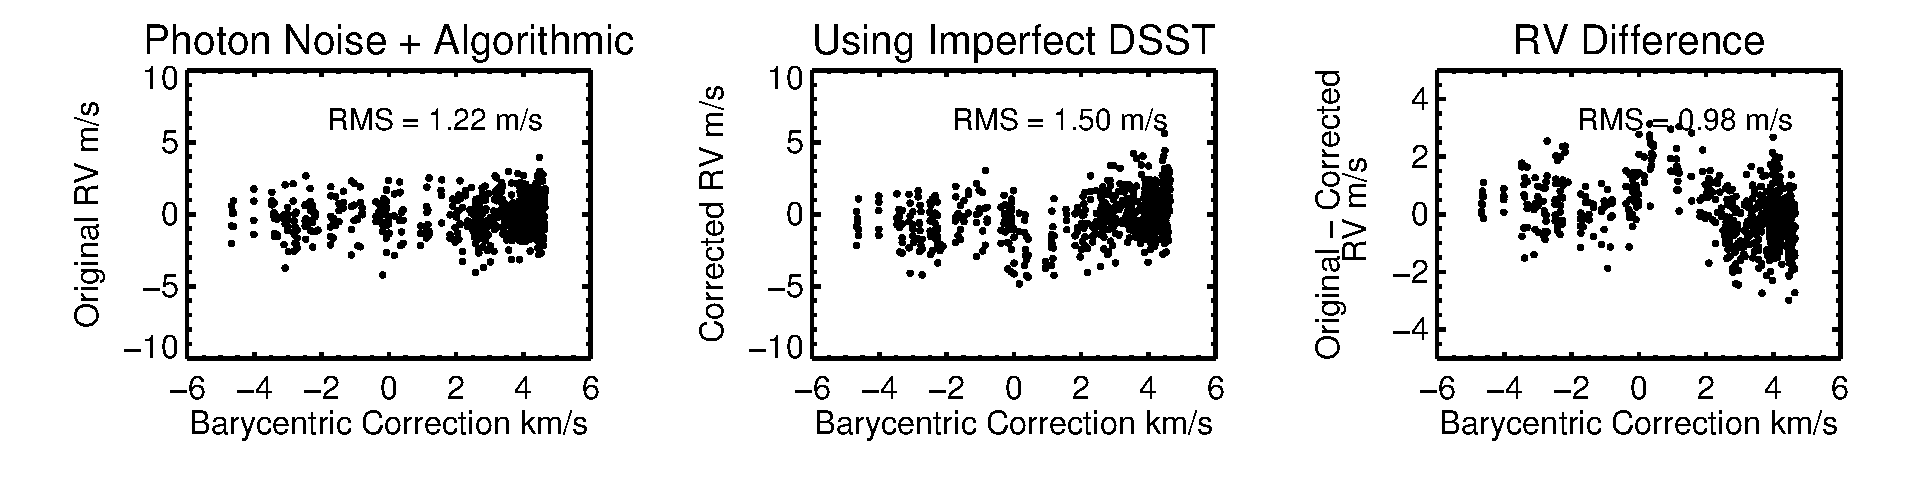
\includegraphics[scale=0.42]{keck/185144-rv-bc-3panel-test0-testd0.eps}}\
\subfloat[HD 10700]{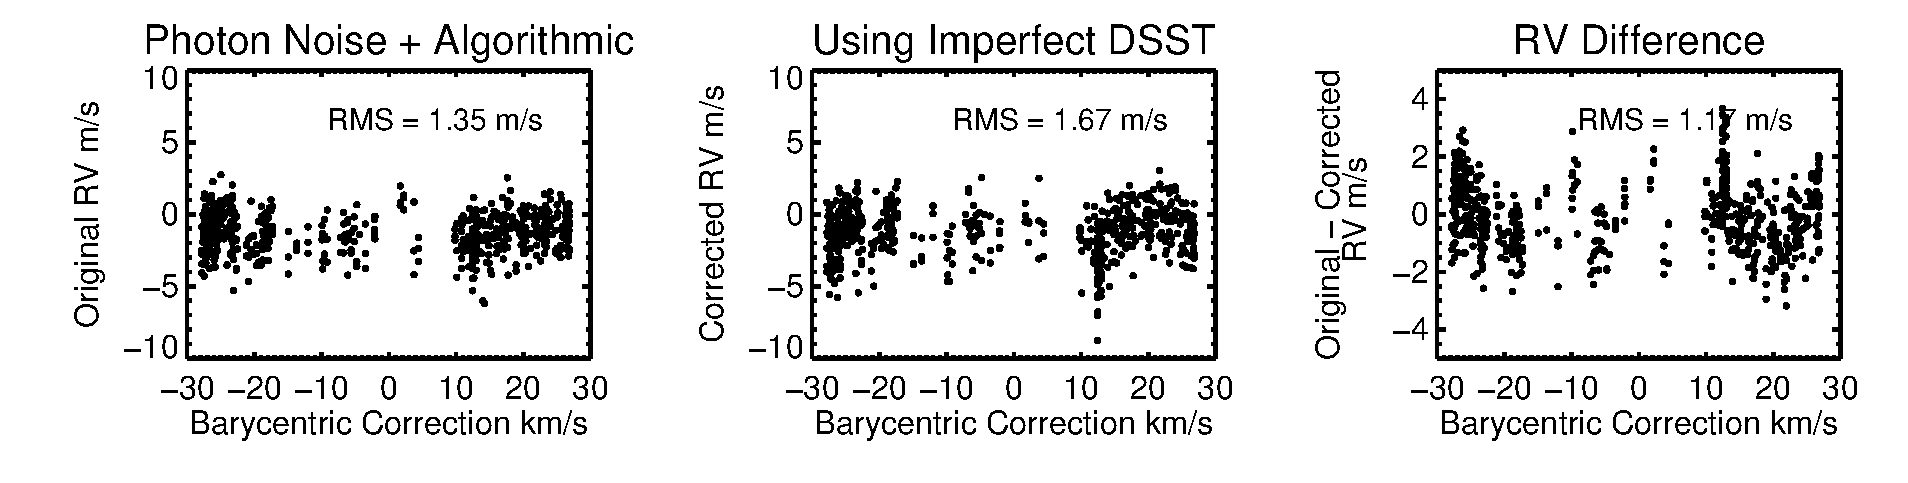
\includegraphics[scale=0.42]{keck/10700-rv-bc-3panel-test0-testd0.eps}}\
\caption{Effect of imperfect DSST on simulated data.
\label{keck:fig:dsst}}
\end{figure}
%----------------------------------------------------------------


%----------------------------------------------------------------
% Chunk illustration of effect of imperfect DSST
% plot made by ~/Exo.../Keck.../simulate.../msplot.pro, plot_name='makefakedsst','chunkcomp'
\begin{figure}
\subfloat{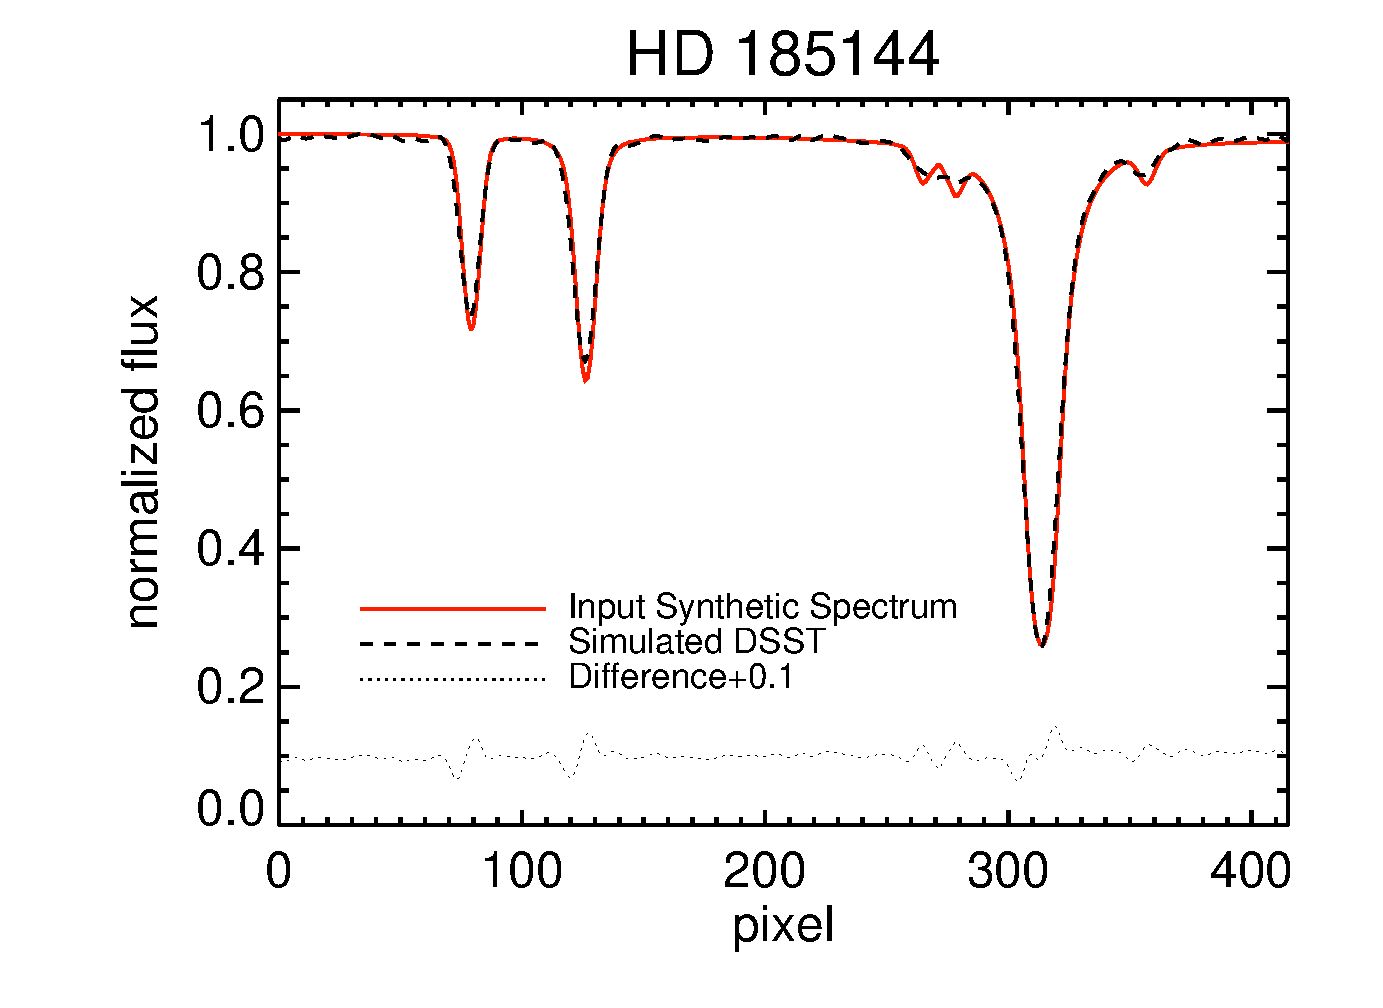
\includegraphics[scale=0.3]{keck/185144_makefakedsst_100.eps}}
\subfloat{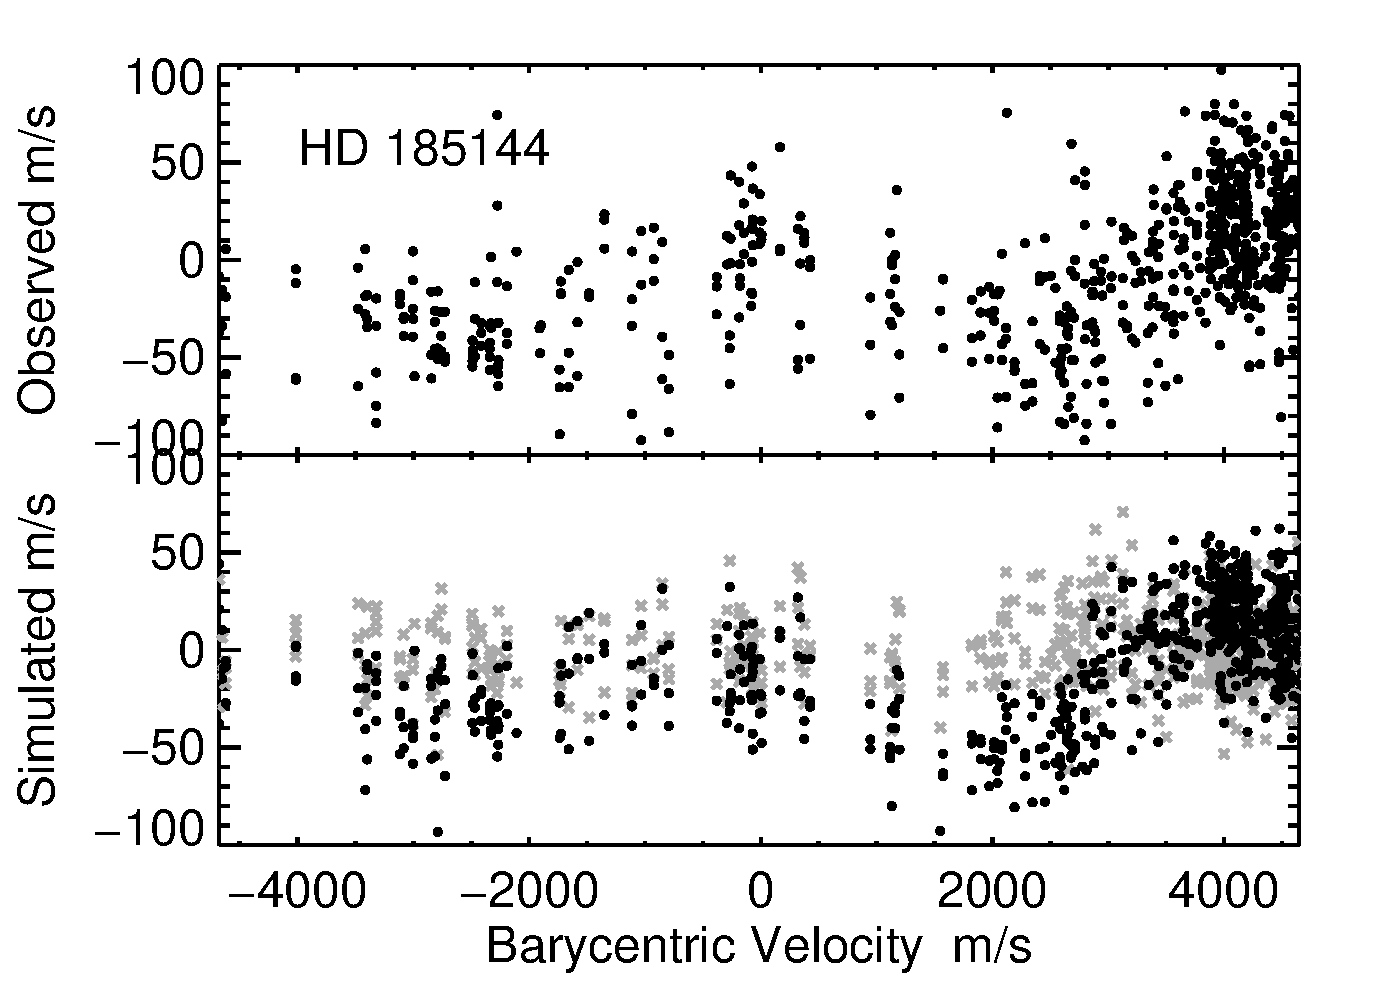
\includegraphics[scale=0.3]{keck/185144_chunkcomp_100.eps}}\
\subfloat{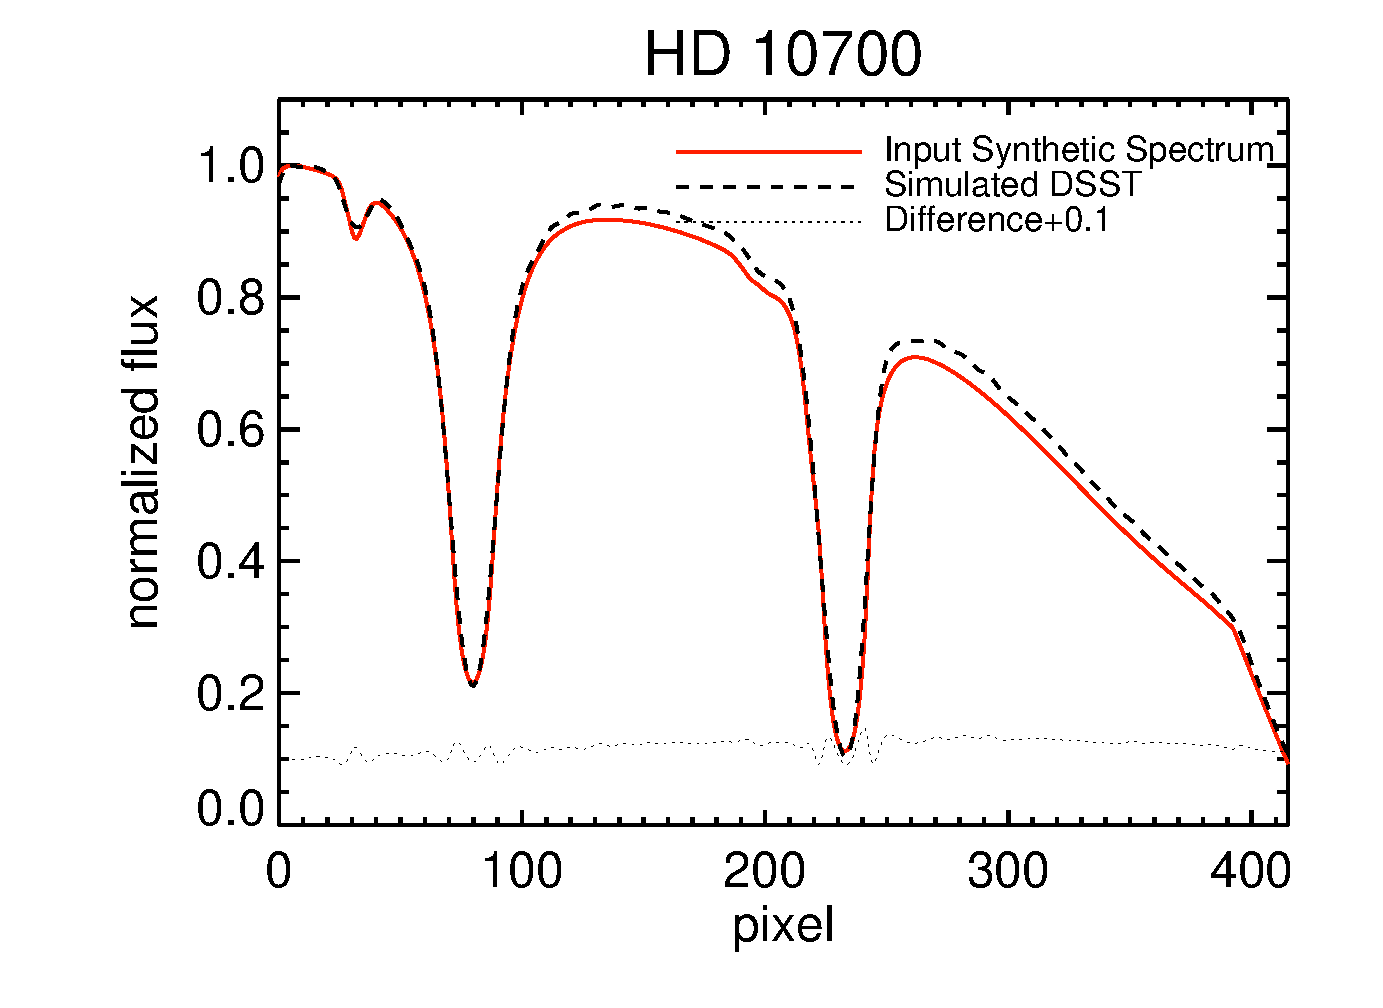
\includegraphics[scale=0.3]{keck/10700_makefakedsst_104.eps}}
\subfloat{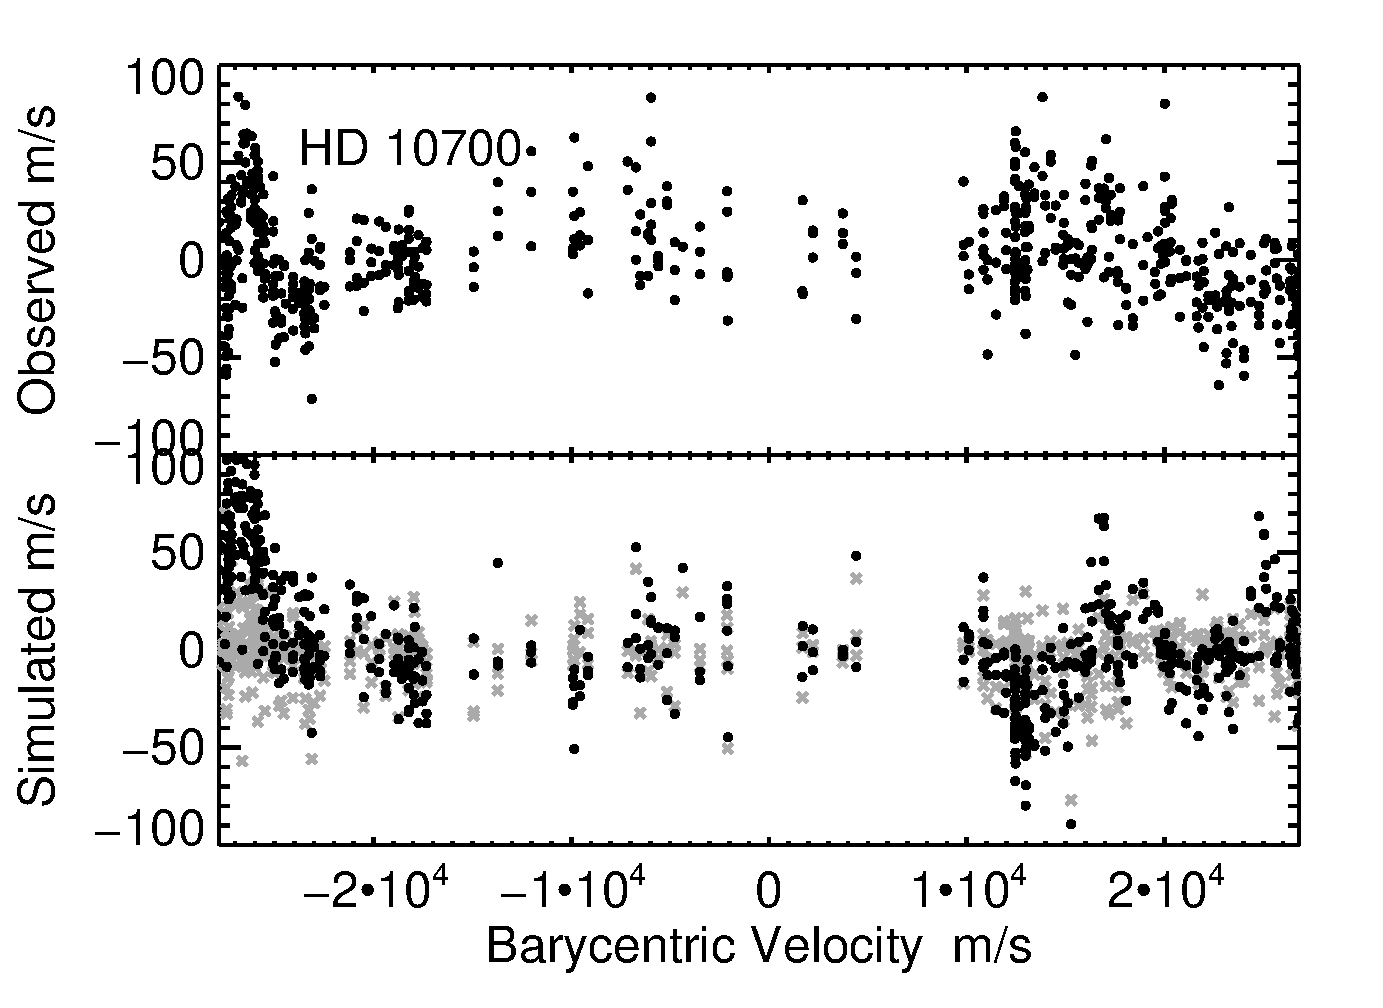
\includegraphics[scale=0.3]{keck/10700_chunkcomp_104.eps}}\
\caption{Effect of imperfect DSST on simulated data for a single
spectral chunk. HD 185144 is for a chunk near 5160\AA, and HD 10700 is
for a chunk around 5166\AA, which are spectral regions that tend to
receive high weights due to ample stellar lines and a lack of telluric
lines.
\label{keck:fig:dsstchunk}}
\end{figure}
%----------------------------------------------------------------




%%%%%%%%%%%%%%%%%%%%%%%%%%%%%%%%%%%%%%%%%%%%%%%%%%%%%%%%%%%%%%%%%%%%%%%%%%%%%%%%
\section{Numerical and Algorithmic Errors}

Solving the least-$\chi^2$ problem in a multi-dimensional, multi-modal
setting is not easy. Efficient as it might be in terms of
computational time, the least-$\chi^2$ algorithm employed by the CPS
Doppler code could give biased solution and comprise the RV precision
and accuracy. We performed simulations to probe the magnitude of such
errors.

Figure~\ref{keck:fig:algorithm} illustrates the RV scatter and RV-BC
trends induced by algorithmic errors -- the RVs plotted are from
simulations with no photon noise added, using the exact input spectrum
as the DSST, and the exact simple Gaussian IPs as the input. A perfect
algorithm should return all zeros for the RV, which is not the case
here. To probe the origin of this algorithmic errors a bit further, we
have run three sets of simulations at three different spectral
resolution (i.e., using different Gaussian IP widths). The amplitude
of the RV scatter decreases as the resolution increases, which is as
expected because shallower spectral lines probably translate to
shallower $\chi^2$ surfaces. However, the signature ``period'' or
length scale (in BC space) of the RV-BC trend does not change, which
is about 8~km/s or 6 pixels on the CCD. We are still investigating the
origin of this signature length scale (perhaps its in the blaze
normalization, or interpolation or rebinning algorithms, to name a
couple). The dichotomy in the red points (the fact that they split
into two RV groups) is probably due to the convergence criteria (which
are tuned for \keck\ resolution, and not sufficient for significantly
higher ones) and the algorithm's sensitivity in initial guesses.


%----------------------------------------------------------------
% Plot showing algorithmic errors
% made by ~/Exo../Keck../simulate.../msplot.pro, in /msplot/.
\begin{figure}
\centering
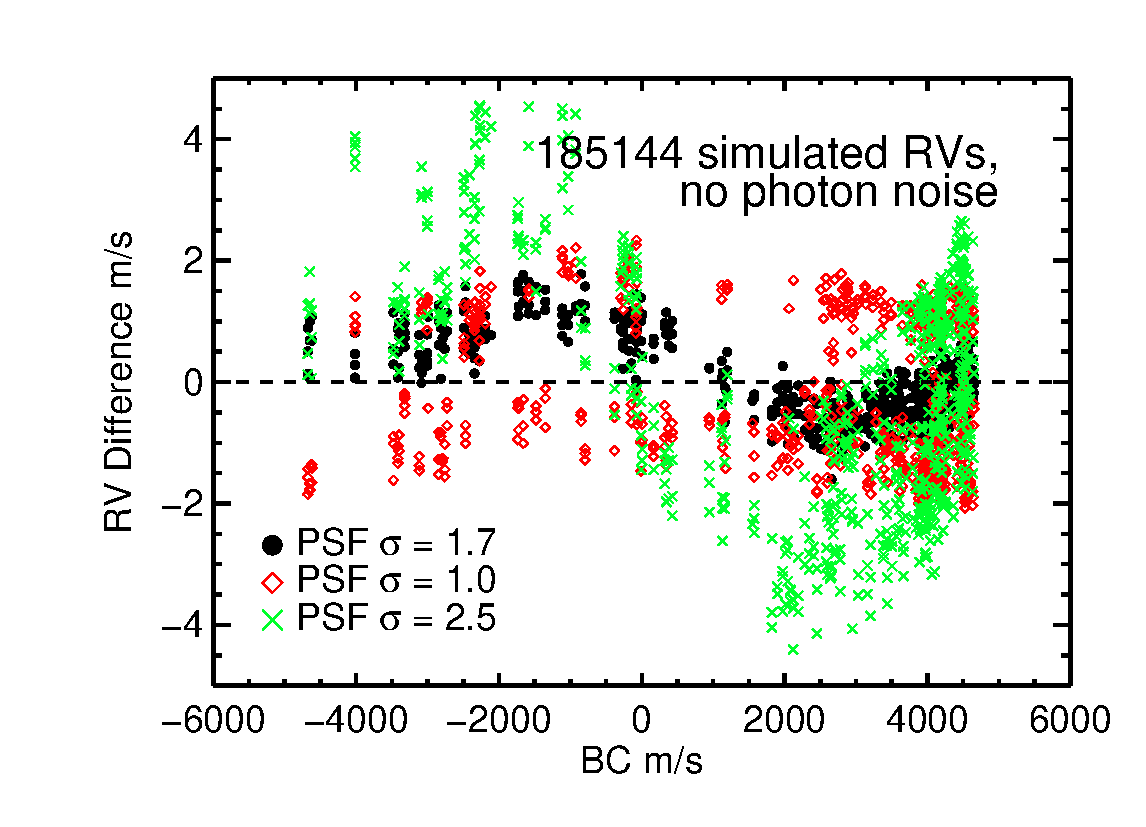
\includegraphics[scale=0.65]{telluric/185144-rv-bc-rja01-rje01-rjf01.eps} 
\caption{RV vs.\ BC for HD 185144, for simulations with fixed simple
IPs and no photon noise added. The data plotted here are from
simulated spectral data with different IP widths (or spectral
resolution, $\sigma=1.7$ pixels corresponds to original \keck\
resolution). The origins of the RV scatters and trends in these plots
are purely algorithmic.
\label{keck:fig:algorithm}}
\end{figure}
%----------------------------------------------------------------

Figure~\ref{keck:fig:chunkalgorithm} shows an example chunk with
visible algorithmic errors. Again the top panel is showing real data,
and the bottom one is the simulated data (with photon noise and
complex IPs). This is a severe case, because its a chunk near 5900\AA\
which does not contain a large amount of stellar or iodine lines, and
therefore it is particularly challenging for the algorithm to find a
good $\chi^2$ minimum.

Unfortunately it is hard to quantify how much RV RMS the algorithmic
errors add to the RV budget, because the major damage comes from the
biases instead of the increased scatter (and the ``vanking'' procedure
breaks down because of this, unable to weigh the chunks effectively
and improve the precision). Figure~\ref{keck:fig:algorithm} suggests
that it can lead to spurious signals with considerable amplitude (1-3
m/s) for high SNR observations (the simulated observations here
essentially have infinitely SNR).


%----------------------------------------------------------------
% Chunk Plot showing algorithmic errors
% made by ~/Exo../Keck../simulate.../msplot.pro, in /msplot/.
\begin{figure}
\centering
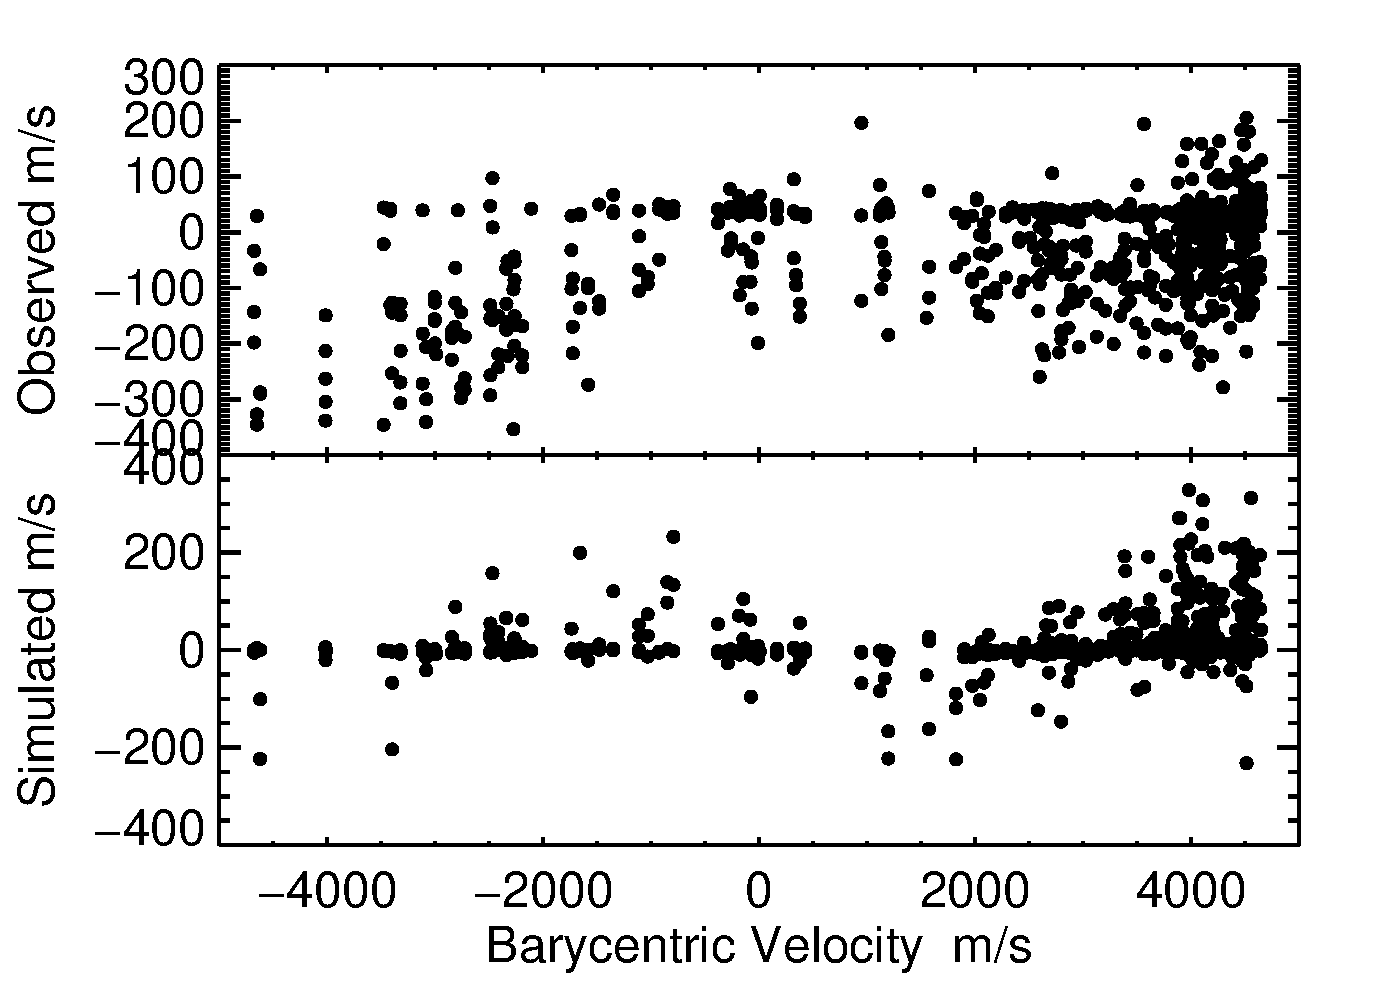
\includegraphics[scale=0.5]{keck/chunkcomp-algorithm.eps} 
\caption{Real (top) or simulated (bottom) Keck RVs from a 2\AA\ chunk
from HD 185144 spectra showing RV systematic errors caused by
algorithmic errors. The RVs in the bottom panel are from the
simulations with complex IPs and photon noise.
\label{telluric:fig:chunkalgorithm}}
\end{figure}
%----------------------------------------------------------------


To list a few places in the Doppler code which may cause significant
numerical and algorithmic errors (not in any particular order): 
\begin{itemize}
\item The LM least-$\chi^2$ fitter: it can get stuck in local
  minima, and it may have reached the crude convergence criteria but not
  actually converged, and it is extremely sensitive to initial guesses.
\item The interpolation algorithm for interpolating or rebinning the model
  spectra. The current algorithm is not flux-conservative.
\item The simple linear fit to the blaze function in each chunk (each
  chunk contains 80 pixels).
\item ``Vanking'', or the final statistical weighting process, only
  takes into account RV scatter of each chunk but not biases.
\end{itemize}

Overall, it is not surprising at all that this decade-old Doppler code
fails to deliver precise RVs to the modern era standard. We discuss
the paths forward in Chapter~\ref{chap:conclusion}.



%%%%%%%%%%%%%%%%%%%%%%%%%%%%%%%%%%%%%%%%%%%%%%%%%%%%%%%%%%%%%%%%%%%%%%%%%%%%
%%%%%%%%%%%%%%%%%%%%%%%%%%%%%%%%%%%%%%%%%%%%%%%%%%%%%%%%%%%%%%%%%%%%%%%%%%%%
\section{Conclusion and Future Work}\label{keck:sec:conclusion}

In this chapter, we described our work on discovering and
characterizing three RV systematic error sources for \keck: telluric
contamination, errors in the DSST, and algorithmic errors. 

Telluric contamination, and in particular, micro-telluric lines, has a
small but non-negligible effects on the RV precision and accuracy. For
a typical G type star like the ones targeted by CPS, micro-tellurics
adds $\sim 0.6$~m/s to the RV error budget (in quadrature) and also a
spurious signal with an amplitude on the order of 10-20~cm/s if left
untreated. We have summarized the best strategies for treating
micro-telluric lines for precise RV using iodine calibrators in
Section~\ref{keck:sec:telluric}, which are masking deep lines,
cleaning DSST, forward modeling the telluric lines in RV extraction,
and assigning lower statistical weights to telluric-contaminated
chunks.

Errors in the DSSTs are one of current major RV systematic sources in
\keck\ RV data, and quite likely the largest one. It adds 1 m/s to the
RV error budget and creates a spurious signal with amplitude $\sim$ 1
m/s. RV-BC trends in simulated data match the ones seen in the
observed spectra among many spectral chunks, which pinned down this
source of error unambiguously. 

Algorithmic errors contribute a considerable amount to the current
\keck\ RV budget as well, and it is hard to imagine it would deliver
sub-m/s precision. After all, it is extremely challenging to find a
$\chi^2$ minimum on a complex surface with 15 dimensions (parameters)
using spectral data with 80 points (80 pixels per chunk) and
highly covariant model parameters. 

In terms of future work along these lines:

{\bf (1) Continuing the battle with telluric contamination: } We plan
to run simulations on an M star, HD 95735, also a RV standard. M stars
are particularly interesting because they may be more susceptible to
telluric contamination -- they have more stellar lines in the red
where the telluric lines are denser. We also plan to implement full
forward-modeling of telluric lines in real data reduction (as opposed
to our toy modeling with fixed water column density for all
dates/observations), and find out whether a priori or floating water
column density parameter works better. We hope to implement our
telluric correction package into the official CPS pipeline eventually,
which will be busily chewing \keck\ follow-up data on TESS targets
(many M dwarfs, undoubtedly) in the near future.

{\bf (2) Searching for a better DSST fabrication method: } We will
diagnose the origin of the DSST errors while searching for a better
deconvolution algorithm. It is possible that the current CPS
``deconvolution'' algorithm described in Section~\ref{keck:sec:dsst}
is sufficient, but the problem is in the normalization or some other
parts of the process. Nonetheless, it could be rewarding to jump out
of the current frame work and try another completely different
approach (e.g., constructing DSST from all the star$+$iodine frames,
which has been attempted by Andrew Vanderberg and John Johnson).

{\bf (3) Eliminating the numerical and algorithmic errors: } The CPS
Doppler code can certainly use an upgrade. However, in order to
eliminate a large portion of the algorithmic errors we are seeing now,
it probably means major structural changes to this lengthy and complex
legacy code written for early-1990 computers, regardless whether one
would like to stick with the L-M least-$\chi^2$ fitter. Therefore,
instead, I am building a new RV extraction code from scratch, using
Python and modern algorithms, which is one of the topics in
Chapter~\ref{chap:conclusion}.



